%%This is a very basic article template.
%%There is just one section and two subsections.
\documentclass{article}

\usepackage{amsmath}
\usepackage{amscd}
\usepackage{amssymb}
\usepackage{amsfonts} 
\usepackage{amsthm}
\usepackage{amsfonts}
\usepackage{amsthm}

\usepackage{circuitikz}
\usepackage{pgf}
\usepackage{tikz}
\usetikzlibrary{arrows,snakes,backgrounds}
% \usetikz
\usepackage{subfig}

\usepackage{algpseudocode}
\usepackage{algorithm}

\usepackage[super]{nth}
% \usepackage{appendix}
% \usepackage{listings}
% \usepackage{color}

\usepackage{hyperref}
%\usepackage{url}

\usepackage{cleveref}
\usepackage{cancel}

\usepackage{aviolov_style}
\usepackage{local_style}


\newtheorem{thm}{Theorem}[section]
\newtheorem{lemma}{Theorem}[thm]
% \theoremstyle{definition}
\newtheorem{ex}{Example}[thm]
\newtheorem{defn}{Definition}[thm]

\begin{document}


\title{stochastic optimal control for spike control in single neurons
\\
---
\vskip5pt
summary
}
\author{Alexandre Iolov 
$<$\href{mailto:aiolo040@uottawa.ca}
		{aiolo040 at uottawa dot ca}$>$, 
		Andr\'e Longtin}

\date{\today}

\maketitle

\abstract{We pose an optimal control problem to precisely specify the spike
timing in a noisy leaky-integrate and fire model of a neuron. The optimal
control problem is solved using Dynamic Programming if the controller has access
to the voltage (closed-loop control) and using a Maximum Principle for the
transition density if the controller only has access to the spike timings (open
loop control)}

\tableofcontents


\section{Introduction}
Neurons relay information by means of voltage spikes - sudden sharp increases in
voltage. Although many details remain unclear, the information content is
thought to be contained in the length of the time-interval between these spikes.
In the simplest case, this can be thought of as a rate-the average number of
spikes per time interval, but more complicated coding schemes are hypothesized to
exist. 

Many experiments allow for manipulating an individual neural cell. A natural
goal then is to make a cell produce a given spike train. This may arise, for
example, in brain-machine interfaces or in artificial prosthetics. 

We now consider this problem in the framework of Stochastic Optimal Control and
give both a feedback solution, when the cell voltage is explicitly and
perfectly observable as well as an open-loop solution when only the occurrence
of a spike is robustly observable. 

The paper is structured as follows: First we describe the neuron model and
formalize the control objective. Then we describe a feedback-based solution
which assumes that the controller has detailed access to the voltage trajectory.
Then we relax the observation assumption so that the controller only has access
to the spike timings. Finally we compare the two methods against a
simple-minded control technique which ignores the stochastic input to the
neuron.

\section{Problem Formulation}
A basic but useful model for a neural membrane potential is the noisy
leaky-integrate-and-fire model:
\begin{equation}
\begin{gathered} 
dX_s = \left(\a(t) - \frac{X_s}{\tc} \right) \intd{s} + \b \intd{W_s},
\\
X(0) = .0,
\\
X(\ts) = \xth \implies  
\begin{cases}
X(\ts^+) = .0 &  
\end{cases}
\end{gathered}
\label{eq:X_evolution_uo}
\end{equation}
In this $X$ represents the membrane electric potential which tries to revert to
$0$ with a time-const of $\tc$, $dW$ is a Brownian motion increment with
intensity $\b$ and $\a(t)$ is our external control. Having last spiked at
time $0$, the potential hits $\xth$ at time $\ts$, we record a spike
of duration $\ts$, the potential resets to $0$ and we start all over again.  

Suppose we want to ensure that spikes occur exactly at the predetermined times
$\tns$ and that we are at least capable of knowing when a spike has occurred.
Then given the renewal nature of our spiking model, we can work sequentially,
focusing only on the first of these intervals, of duration $t_1 = \T$, and then
ask: how do we choose $\a(t)$ st. $\ts = \T$. A natural optimal control
objective formulating this is to require a least squares solution
\begin{equation}
\a(t) = \argmin_{\a(t)} \{\, \Exp[(\ts- \T)^2] \,\}
\label{eq:OC_LS_variance}   
\end{equation}
where expectation is taken with respect to the trajectories of $X_t$.

It is also natural to assume that our control has certain limitations. The
simplest and most common are simple bounded constraints:
\begin{equation}
\a(t) \in [\amin, \amax] \quad \forall t
\label{eq:bound_constraints_alpha}
\end{equation}

% \subsection{Optimal Control Formulation}
In addition to \cref{eq:OC_LS_variance}, our objective will also contain a
running cost based on the control. This regularizes the problem eliminating the
subtleties of singular-control situations and it might be argued appropritate
to avoid excessive control.

So we will seek an optimal control, $\a$ that solves:
\begin{equation}
\a(t) = \argmin_{\a(t)} \Big\{ \,
\Exp\left[
\e \int_0^\ts  \a^2 \intd{s}
+  
(\ts - \T \big)^2 \right]  \, \Big\}
\label{eq:OC_LS_variance_energy}   
\end{equation}
where $\e$ measure how much weight we put on minimizing the energy expenditure
and if $\e \rightarrow 0$, then we do not care at all.
  
We will consider two scenarios, one, {\sl closed loop control}, in which the
value of $X_t$ at $t$ is known and can be used in determining the control and
,two, {\sl open loop control} in which only the times of spikes is known. In
closed-loop scenario, we might better write the control as
$$\a = \a(x,t)$$ to indicate its dependence on $X_t$. In the open-loop scenario,
we would instead write $$\a = \a(t)$$ to indicate that we will always do the
same thing regardless of the (unknown) behavious of $X_t$. The techniques used
in both scenarios will be different. For the closed-loop scenario we will use Dynamic Programing,
\cite{Fleming1975}, while for the open-loop scenario we will use a form
of the Maximum Principle for transition densities, \cite{Ahmed1981}.

Crucially, we assume that the model parameters in \cref{eq:X_evolution_uo} are
known and given.

\section{Closed-Loop Solution - Dynamic Programing}
Given $t, X_t = x$, let $\t$ be the (unknown) remaining time to spike. For
example, given $t=0, X=.0$, $\t = \ts$, the entire duration of the inter-spike interval.
Starting from a general $t, x$, our remaining-cost objective, $J[\a; x,t]$,
will be:
\begin{equation}
J[\a, x,t]  = \Big\{ \,
\Exp\left[
\e \int_t^\ts  \a^2 \intd{s}
+
(\t - (\T-t) \big)^2 |x,t
\right] \, \Big\}
\label{eq:OC_LS_mean_objective}   
\end{equation}
i.e.\ if time $t$ has elapsed without a spike, we now want to minimize
the difference between $\t = \ts - t$ and ($T-t$), given the current state $x$.
Recall that in the closed-loop scenario, we assume that $x = X_t$ is known
to the controller. 

\subsection{Hamilton-Jacobi-Bellman equation for the value function}
We are now in a position to set up the Hamilton-Jacobi-Bellman (HJB) equation
\cite{Fleming1975,Evansb} for this problem. First introduce the value function,
$v(x,t)$ as: 
\begin{align}
v(x,t) =& \argmin_{\a(s \geq t)} \{J[\a, x,t] \}
\notag 
\\ 
=&
\argmin_{\a(s \geq t)} 
\Big\{ \,
\Exp\left[
\e \int_t^\ts  \a^2 \intd{s}
+
(\t - (\T-t) \big)^2 |x,t
\right] \, \Big\}
\label{eq:OC_LS_mean_value}   
\end{align}

The corresponding HJB PDE for $v$ is:
\begin{equation}
\di_t v(x,t) + \tfrac{\b^2}{2} \di_x^2 v + \min_{\a \in [\amin, \amax]}\big\{
\e \a^2 + (\a-\tfrac{x}{\tc}) \di_x v \big\} = 0
\label{eq:OC_LS_mean_HJB}
\end{equation}

In this set-up we can solve for the optimal control analytically via:
\begin{align}
\a(x,t)  =&\argmin_{\a \in [\amin, \amax]}\big\{
\e \a^2 + (\a-\tfrac{x}{\tc}) \di_x v \big\}
\notag 
\\
=& 
\min \left(\amax, \max\left(\amin, -\frac{\di_x v}{2\e}\right)
\label{eq:OC_LS_variance_energy_quadratic_control}
\end{align}
With this the HJB becomes
\begin{equation}
\di_t v(x,t) + \tfrac{\b^2}{2} \di_x^2 v + 
\e (\astar)^2 + (\astar-\tfrac{x}{\tc}) \di_x v 
= 0
\label{eq:OC_LS_mean_HJB_bounded_control}
\end{equation}

Now, we need to consider boundary conditions (BCs). If $X_t =
\xth$ then we have a spike now and we know that $\ts = t$. Thus:
$$
v(\xth,t) = (t-\T)^2
$$
Now for $x \ll .0$, we can assume that $v$ doesn't really depend on $x$ so say 
$$
\di_x v(\xmin, t) = .0
$$
This is legitimate if we impose artificial reflecting boundaries for the
diffusion at $\xmin$. So we need to determine for which $\xmin$ is a reflecting
boundary consistent with the dynamics. For example, we can take $\xmin$ to be
two standard deviations of the stationary distribution of the non-controlled, $\a=0$, \cref{eq:X_evolution_uo}.
% Ooops,
% we need $\di_x v \neq 0$ and here we are setting $\di_x v = 0$ in one of the BCs\ldots oh well.

Finally we come to the Terminal Conditions (TCs) for $v$. The idea is simple: if
we reach $\T$ without having spiked we will just apply maximum control in
the positive direction, i.e.\ $$t>T \implies \a(t) =
\amax$$ Thus: $$ v(x,T) = \Exp[\t^2|x, \amax] $$. This is indeed optimal only if
we ignore the energy term, $\eps u^2$ in the objective, and is a good
approximation for $\epx \ll 1$.

Thus we restate the HJB equation in its fully specified form:
\begin{equation}
\begin{gathered}
\di_t v(x,t) + \tfrac{\b^2}{2} \di_x^2 v + 
\e \a^2 + (\a -\tfrac{x}{\tc}) \di_x v 
= 0
\\
\a (x,t) = \min \left(\amax, \max\left(\amin, -\frac{\di_x v}{2\e}\right)
\right)
\\
\begin{cases}
v(\xth,t) = (t-\T)^2  \quad & \textrm{upper BC}
\\
\di_x v(\xmin, t)  = .0  \quad &\textrm{lower BC}
\\
v(x,T)  = \Exp[\t^2|x, \amax]  \quad& \textrm{TC}
\end{cases}
\end{gathered}
\label{eq:OC_LS_HJB_full}
\end{equation} 
We are solving $v(x,t)$ over $[\xmin, \xth] \times [0,T]$.

A few words on the terminal conditions (TCs). $\Exp[\t^2|x, \amax]$ is the
expected time to spike (reach the threshold) starting at $x$ and applying
$\amax$ throughout. We will not show it here, but this quantity can be found
easily for all $x$ in the domain by solving a stationary backward Kolmogorov
equation. 

\subsection{Solving the HJB - the numerical method for
\cref{eq:OC_LS_mean_HJB_bounded_control}}
We now have a PDE for $v$ and an algorithm for computing all the BCs and TCs of
this PDE. It is time to discuss the numerical method for solving
\cref{eq:OC_LS_HJB_full}. Since we are in 1-d the simplest thing to do is try a
centred Finite Difference scheme, upwind wherever necessary and hope for the
best.

We will not discuss a detailed study of the convergence properties of the
numerical method, but just demonstrate its performance on a representative
parameter set in \cref{fig:HJB_attempt}. 

Let us discuss the most salient features of \cref{fig:HJB_attempt}. At the end,
when $t = \T$, the value function, $v$ is monotonely decreasing. This makes
sense, becaue the lower $x$ is the more time on average will it take us to spike
and the more delay will we have from our desired spike time. However, as we go
back in time $v$ inverts, in the sense that for $t \ll \T$, we would like to
be somewhat far from the boundary to avoid the risk of spiking early.

Now focus on the controls, \cref{fig:HJB_attempt_control}: Naturally, at the
end we have the control assume its maximum value, $\a(t>=\T) = \amax$. As we
start to go back in time however, two things start to happen, the control $\a$
decreases for $x \ll \xth$, and it becomes negative for $x \lesssim \xth$. 
That is fully consistent with the problem objective - for
$t<\T$, we want to distance $X_t$ from the threshold to avoid an early spike.
\begin{figure}[h!]
\begin{center}
\subfloat[Solution, $v$]
{
\label{fig:HJB_attempt_soln}
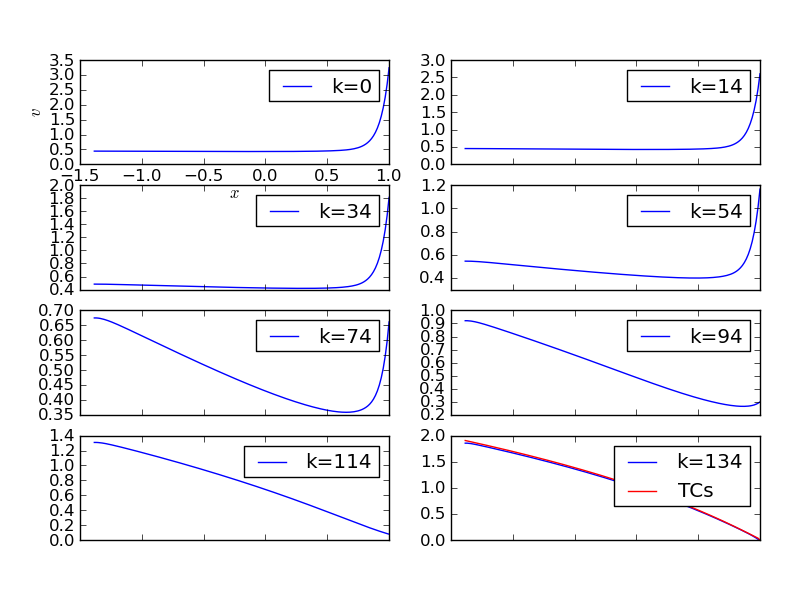
\includegraphics[width=0.48\textwidth]
{Figs/HJB/soln_al=-20_au=20__t=5_b=8.png}
}
\subfloat[Controls, $\a$]
{
\label{fig:HJB_attempt_control}
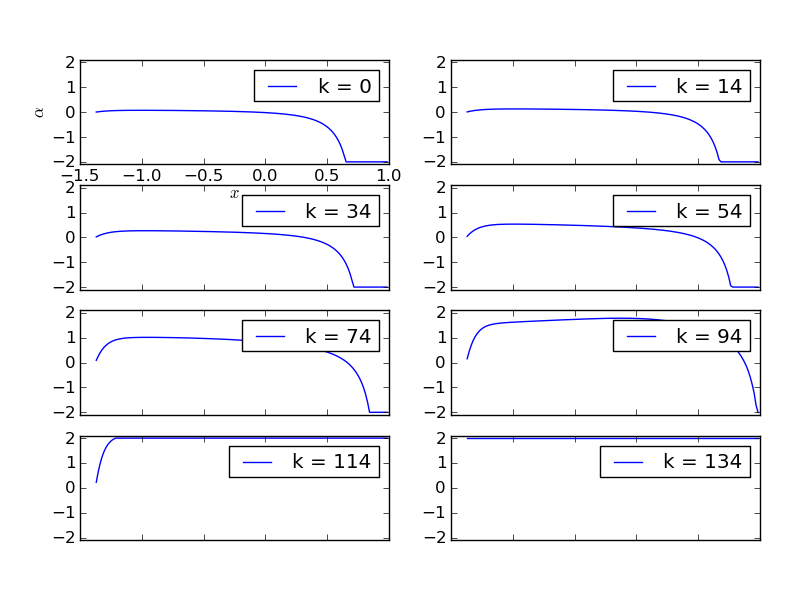
\includegraphics[width=0.48\textwidth]
{Figs/HJB/control_al=-20_au=20__t=5_b=8.png}
}
\caption[]{The solution and controls for the HJB PDE parametrized by:
$\tc = 0.50,  \beta = 0.75,
\amin = -2.00, \amax = 2.00, \eps=0.10,
\T = 1.80$. The $k$ index indicates the time-step, and recall that we are
running backwards in time, so the computation actually happens from right-to-left, bottom-to-top}
\label{fig:HJB_attempt}
\end{center}
\end{figure}

\section{Open-loop Stochastic Control}
As we have mentioned before, when the value of $X_t$ is unknown , the best one
can do is to use the transition density to perform the optimization. Since the
transition density follows a (deterministic) PDE, we will thus apply a Maximum
Principle for PDEs as a method of obtaining the optimal
control, \cite{Ahmed1981,Borzi2012}.

\subsection{Fokker-Planck equation for the state density evolution} 
We will need the transition density of $X$, conditional on no
spikes having occurred. We will write this as:
\begin{align*}
f(x,t) \intd{x} &= \Prob[X_t\in \intd{x} | X_0 = .0, X_{s<t} < \xth]  								  
\end{align*}
Then $f$ satisfies a Fokker-Planck equation with absorbing boundaries
\begin{equation}
\begin{gathered}
\di_t f(x,t) =
				\frac{\b^2 }{2}\cdot \di^2_x f -  
				\di_x \Big[ \left(\a(t)- \frac{x}{\tc}\right)  \cdot f \Big]
\\
\\
\begin{array}{lll}
	&\textrm{st.\ }& 
	\left\{ \begin{array}{lcl}
	 f(x,0) &=& \delta(x) \quad \textrm{delta function}
	\\
	(\a(t)- \tfrac x \tc)f - \di_x \tfrac {\b^2}2 f] \big|_{x=\xmin} &\equiv& 0
	\quad \textrm{reflecting BCs at some } \xmin 
	\\
	f(x,t) |_{x=\xth} &\equiv& 0 \quad \textrm{absorbing BCs at } \xth
\end{array} \right. 
\end{array}
\label{eq:FP_pde_OU_PDF}
\end{gathered}
\end{equation}
In theory, $\xmin = -\infty$, but in the numerics below we will need to
truncate it to some finite value, exactly as in the HJB equation,
\cref{eq:OC_LS_HJB_full}.

The $f$ dynamics can also be written as
$$
\di_t f(x,t) = - \di_x \phi(x,t)
$$
for the probability flow, $\phi$, 
$$
\phi(x,t) = (\a- \tfrac x \tc)f - \di_x [\tfrac {\b^2}2 f]
$$
Then the lower BC is
$$
\phi(x,t) |_{x=\xmin} \equiv 0
$$

We will also need a short hand notation for the differential operator on the
right side of \cref{eq:FP_pde_OU_PDF}. Let $$ \L_\a[\cdot] := \di^2_x [
\frac{\b^2 }{2} \cdot] - \di_x  [ (\a(t)- \frac{x}{\tc}) \cdot] $$ We will
usually omit the subscript $\a$, but have written it now, since the operator is
parametrized by $\a$, that is by the control.


\subsection{Restating the objective in terms of $f$}
Let us recall our objective, \cref{eq:OC_LS_variance}:
$$
J(\a) = \Exp\left[
(\ts - \T \big)^2 
+  
\e \int_0^\ts  \a^2(s) \intd{s}
\right]
$$
Rewriting this in terms of $f$ reads:

\begin{align}
J(\a) =& 
\int_\xmin^\xth \Exp[\t^2|x, \amax] \cdot f(x,\T) \intd{x}
\notag
\\
&+ \int_0^\T \phi(\xth, t) (t-\T)^2 \intd{t}
\notag
\\
&+  \e \int_0^\ts  \a^2(t)  \int_\xmin^\xth f(x,t) \intd{x} \intd{t}
\label{eq:OC_LS_variance_density}
\end{align}
Let us explain in more detail each term on the RHS in
\cref{eq:OC_LS_variance_density}.

The first term $$ \int_\xmin^\xth \Exp[\t^2|x, \amax] \cdot f(x,\T) \intd{x} $$
counts the cost of trajectories which spike too late. This cost is the expected
squared time-to-hit starting at $x$, with  $\a = \amax$, weighted by the
probability of $X_\T = x$, which is just $f(x,\T)$.

The second term
$$
\int_0^\T \phi(s,t) (t-\T)^2 \intd{t}
$$
counts the cost of trajectories which spike too soon, that
is the squared difference between realized spike time, $t$ and desired spike
time $\T$, weighted by the probability of spike at $t$ which is just the outflow of
probability, $\phi(\xth,t)$. Note further that due to the homogeneous
Dirichlet BC on $f$ at $\xth$, the outflow is simply:
$$
\phi(\xth, t) = -\frac{\b^2 }{2} \di_x f(\xth, t) 
$$

Finally, the third term
$$
\e \int_0^\ts  \a^2(t)  \left[  \int_\xmin^\xth f(x,t) \intd{x} \right] \intd{t}
$$
is the energy cost: the inner integral, $\int_\xmin^\xth f(x,s) \intd{x}$
takes into account that we incur an energy cost only for those trajectories
which have not yet spiked.

With that our control $\a$ will naturally be found via:
$$
\a = \argmin J[\a]
$$

\subsection{Optimizing with $f$ using a Pontryagin-type Maximum Principle}
\label{sec:PDE_max_principle_for_pdf}
By now our ostensibly stochastic optimal control problem modelled by SDEs
has become a deterministic optimal control problem modelled by PDEs. Our control
$\a$ influences the evolution density $f$ and via $f$, the integrals in the
objective, $J$.

The Maximum Principle introduces an adjoint variable, $p$, which solves a PDE
related to the PDE satisfied by the density $f$ and then calculates the optimal
control, $\a$ as a function(al) of $f$ and $p$.

In short, the equation for the adjoint, $p$, is 
\begin{equation}
\begin{gathered}
\begin{aligned}
\di_t p =& - \Lstar[p]
\\
		=&  
			- \Big[ \frac{\b^2 }{2}\cdot \di^2_x p +  
			(\a(t)- \frac{x}{\tc})  \cdot \di_x p \Big] 
\end{aligned}
\\
\st  
\begin{cases}
	p(x,\T) &= \Ttwo(x)
	\\ 
	\di_x p  \big|_{x=\xmin} &\equiv 0
	\\
	p \big|_{x=\xth} &\equiv (s-T)^2
\end{cases}
\label{eq:adjoint_pde_OU}
\end{gathered}
\end{equation} 

and then $\a$ can be found via
\begin{equation}
\Big\{
 \tilde{\e}  2 \a(t)
+ p f \Big|_\xmin
- \int _\xmin^\xth p \cdot \di_x f \intd{x} 
\Big\} = 0
\quad \forall t \in [0,T]
\label{eq:J_necessary_condition}
\end{equation}

More practically, the quantity, 
$$\di_\a J =  \Big\{
 \tilde{\e}  2 \a(t)
+ p(x,t) f(x,t) \Big|_\xmin
- \int _\xmin^\xth p \cdot \di_x f(x,t) \intd{x} 
\Big\}
$$
gives us the direction of increase of $J$ at $\a(t)$
and we can use it as a gradient in a descent algorithm, given some initial
guess, $\a_0(t)$, for the control.

Finally, we are ready to calculate the open-loop stochastic optimal control for
this parameter set. The results are in
\cref{fig:FP_adjoint_objective_control_convergence}.
\begin{figure}[h]
\begin{center}
\subfloat[$\a_k(t)$ ]
{
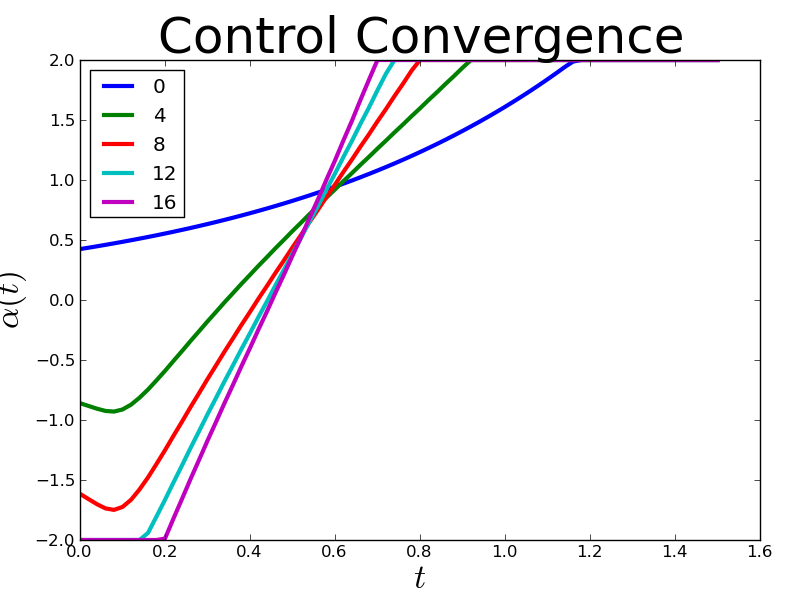
\includegraphics[width=0.48\textwidth]
{Figs/FP_Adjoint/ExampleControlConvergence_control.png}
}
\subfloat[$J_k$ ]
{
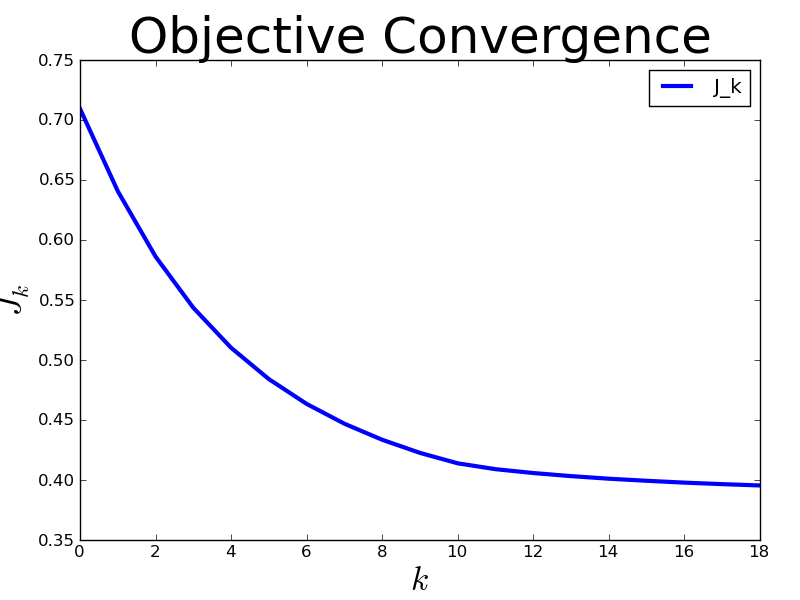
\includegraphics[width=0.48\textwidth]
{Figs/FP_Adjoint/ExampleControlConvergence_objective.png}
}
\caption[ ]{The result of an entire optimization iteration, on the left the
iterates of the control, $\a_k(t)$, on the right the progress of the
objective with each iteration. The final control, in purple, is inhibitory at
the beginning of the time interval, $\a < 0$, unlike the the deterministic
control solution. 
We see a significant
reduction in the objective value, $J$, and thus an improvement, on the
order of 50\%.}
\label{fig:FP_adjoint_objective_control_convergence}
\end{center}
\end{figure}

% \begin{table}[h] 
% \centering
% \begin{tabular}{lc}
% Control Law & Squared Error \\
% \hline
% Deterministic &  0.647 \\
% Stochastic &  0.336\\
% Theory (Value function) & 0.285
% \end{tabular}
% \caption{Realized performance of the different control laws and the theoretical
% expected performance of the stochastic law (last row)}
% \label{tab:realized_avg_errors_det_vs_stoch}
% \end{table}
% 
% \begin{figure}[h]
% \begin{center}
% \subfloat[A]
% {
% \label{fig:controlled_traj_ex1}
% \includegraphics[width=0.33\textwidth]
% {Figs/ControlSimulator/example_controlled_trajectories_id1.png}
% }
% \subfloat[B]
% {
% \label{fig:controlled_traj_ex2}
% \includegraphics[width=0.33\textwidth]
% {Figs/ControlSimulator/example_controlled_trajectories_id4.png}
% }
% \subfloat[C]
% {
% \label{fig:controlled_traj_ex3}
% \includegraphics[width=0.33\textwidth]
% {Figs/ControlSimulator/example_controlled_trajectories_id3.png}
% }
% \caption[]{Examples for the controlled trajectories using both the deterministic
% and the stochastic control approaches. The red vertical line in the plots
% indicates the desired spike-time, $\T$. In A, B the performance of both
% control laws is essentially the same, but in C we see the advantage of the
% stochastic approach. $\tc, \b = [.75, 1.25]$.}
% \label{fig:control_trajectories_examples}
% \end{center}
% \end{figure}
% \begin{figure}[htp]
% \begin{center}
%   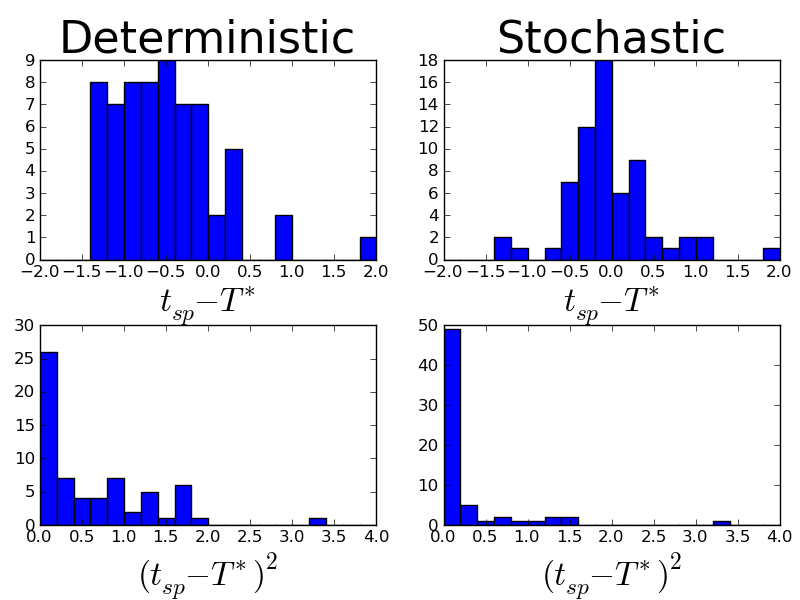
\includegraphics[width=.9\textwidth]{Figs/ControlSimulator/example_controlled_trajectories_hists.png}
%   \caption[labelInTOC]{Histogram of the spike timing error for the
%   deterministic (left) vs. the stochastic (right) control laws.}
%   \label{fig:error_histograms_det_vs_stoch}
% \end{center}
% \end{figure}


\section{Test Comparison of Different Controls}
\label{sec:probabilistic_numerical_test}
We now compare the performance of the optimal closed-loop and open-loop controls
as well as a very naive open-loop controller, which is obtained by assuming
$\b=0$. This naive controller is called 'Deterministic', since it assumes
deterministic dynamics in $X_t$. 

For the comparison we sample $128$ realizations of the controlled system
and apply in turn each of the three controls.

We set $\e = .001$ and $\amax = 2.0$. As such the energy cost is of
secondary importance and the paramount effect on the objective is the difference
$(\ts - \T)$, which we are trying to minimize. We set $\tc, \b = [.75, 1.25]$.

The performance of the three controllers is given in
\cref{tab:realized_avg_errors_det_vs_openloop_vs_stoch}. We see that while the
open-loop stochastic control is not as good as the feedback stochastic
control, it is much closer in performance to it than to the naive
deterministic control.

For illustration sake, we also show the error
histograms in \cref{fig:error_histograms_det_vs_openloop_vs_stoch} and visualize
some trajectories in \cref{fig:control_trajectories_examples}.

\begin{table}[h] 
\centering
\begin{tabular}{lcc}
Control Law & Squared Error &  Squared Error \\
 & Empirical & Theoretical\\
\hline
Deterministic &  0.621 & - \\
Open-Loop Stochastic & 0.356 & 0.382\\
Feedback Stochastic &  0.288& 0.285\\
\hline
\end{tabular}
\caption{Realized and theoretical performance of the different control laws. The empirical
performance is obtained using 128 sample paths. The theoretical performance is
found using the $J$ in for the open-loop stochastic control and the value
function $v(x=0, t =0)$ for the closed-loop stochastic control.}
\label{tab:realized_avg_errors_det_vs_openloop_vs_stoch}
\end{table}
\begin{figure}[h]
\begin{center}
\subfloat[]
{
\label{fig:controlled_traj_ex1}
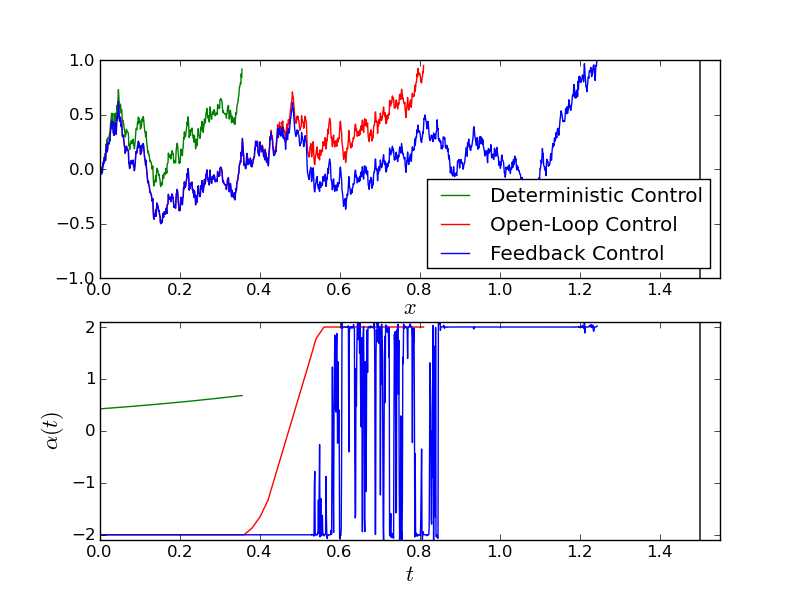
\includegraphics[width=0.33\textwidth]
{Figs/ControlSimulator/3controls_example_trajectories_id3.png}
}
\subfloat[ ]
{
\label{fig:controlled_traj_ex2}
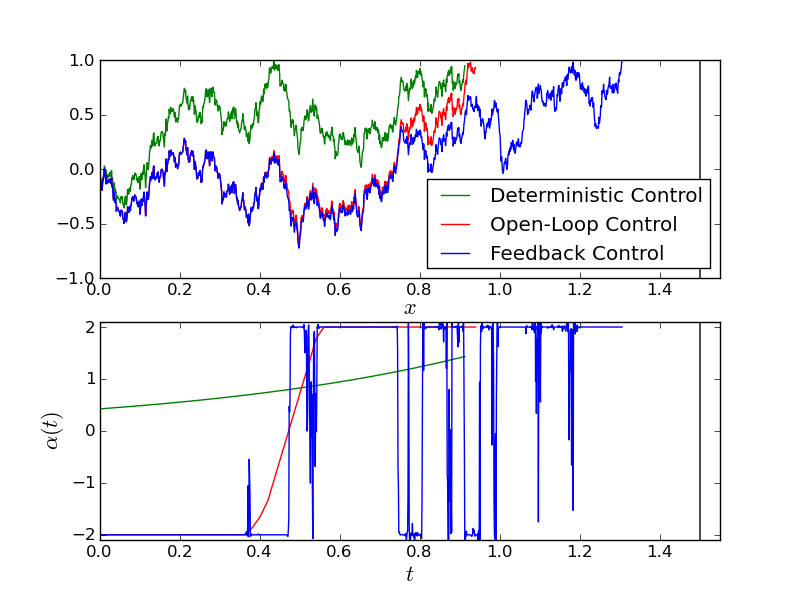
\includegraphics[width=0.33\textwidth]
{Figs/ControlSimulator/3controls_example_trajectories_id5.png}
}
\subfloat[ ]
{
\label{fig:controlled_traj_ex3}
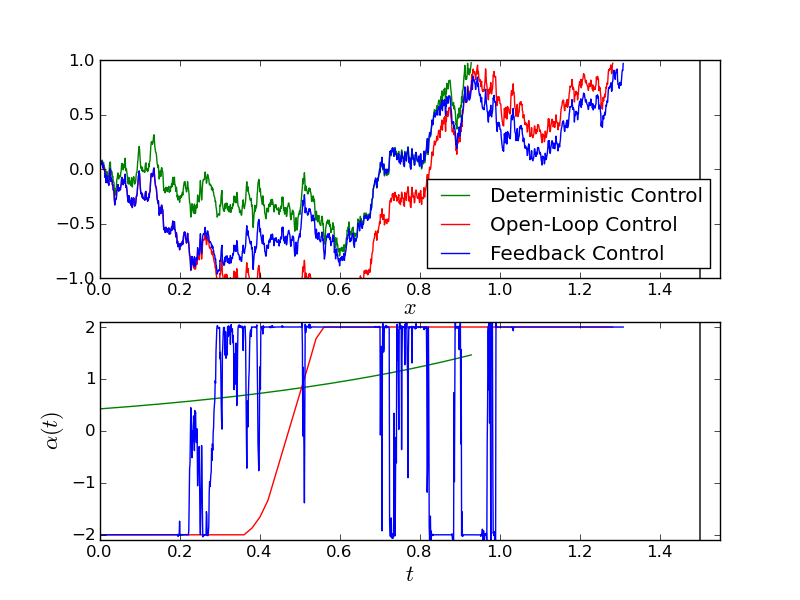
\includegraphics[width=0.33\textwidth]
{Figs/ControlSimulator/3controls_example_trajectories_id6.png}
}
\caption[]{Examples for the controlled trajectories using the deterministic,
open-loop stochastic and feedback stochastic control approaches. The
black vertical line in the plots indicates the desired spike-time, $\T$.
For the parameter values are $\tc, \b = [.75, 1.25]$. The three panels are
three different realizations of the model dynamics.}
\label{fig:control_trajectories_examples}
\end{center}
\end{figure}

\begin{figure}[h]
\begin{center}
  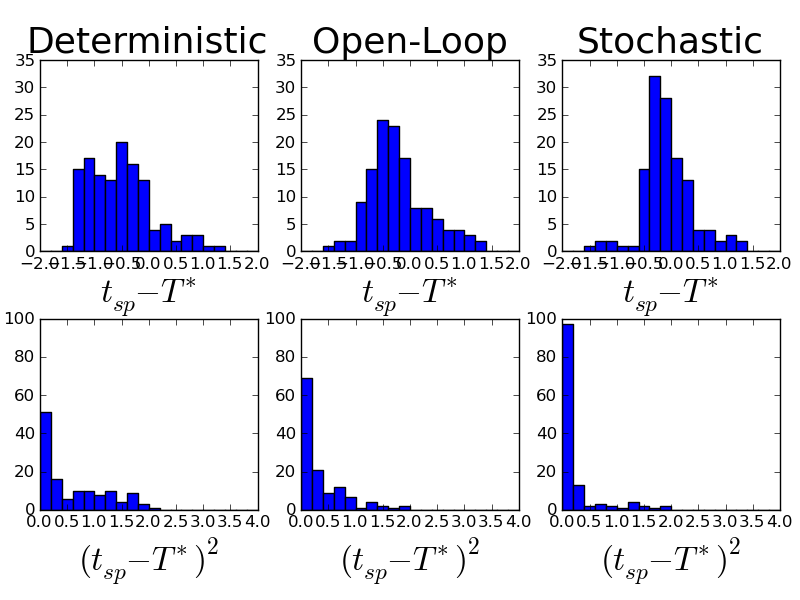
\includegraphics[width=.95\textwidth]
  {Figs/ControlSimulator/3controls_example_trajectories_hists.png}
  \caption[labelInTOC]{Histogram of the spike timing error for the
  deterministic (left) vs. open-loop stochastic(centre) vs. feedback stochastic
  (right) control laws. This is for the same problem as in
  \cref{fig:control_trajectories_examples}. We have used $N=128$ sample paths
  to form the statistics}
  \label{fig:error_histograms_det_vs_openloop_vs_stoch} 
\end{center}
\end{figure}

\bibliographystyle{plain}
\bibliography{library}

\end{document}
